\documentclass{lposter}
\usepackage{graphicx}
\usepackage{natbib}
\usepackage{booktabs}
\usepackage{subfig}
\usepackage{amsmath}
\usepackage{alltt}
\usepackage{textcomp}
\usepackage{url}
\usepackage{amssymb, amsthm, bm}
\usepackage{semantic}

\bibliographystyle{alpha}

\theoremstyle{plain}
\newtheorem{theorem}{Theorem}
\newtheorem{lemma}{Lemma}
\newtheorem{prop}{Proposition}
\newtheorem{rem}{Remark}
\newtheorem{cor}{Corollary}

\theoremstyle{definition}
\newtheorem{definition}{Definition}
\newtheorem{ex}{Example}

\newcommand{\Z}{\mathbb{Z}}
\newcommand{\N}{\mathbb{N}}
\newcommand{\F}{\mathbb{F}}
\newcommand{\R}{\mathbb{R}}
\newcommand{\C}{\mathbb{C}}
\newcommand{\Q}{\mathbb{Q}}
\newcommand{\E}{\mathbb{E}}
\newcommand{\OC}{\mathcal{O}}
\newcommand{\bi}{\textbf{i}}

\renewcommand{\tt}[1]{\texttt{#1}}
\newcommand{\tts}[1]{\tiny{\texttt{#1}}}
\definecolor{ao(english)}{rgb}{0.0, 0.5, 0.0}
\definecolor{babyblue}{rgb}{0.54, 0.81, 0.94}
\newcommand{\agent}[1]{{\color{ao(english)}#1}}
\newcommand{\activity}[1]{{\color{babyblue}#1}}
\newcommand{\dataset}[1]{{\color{yellow}#1}}

\newcommand{\red}[1]{{\color{red}#1}}
\newcommand{\green}[1]{{\color{green}#1}}
\newcommand{\blue}[1]{{\color{blue}#1}}
\newenvironment{myprogramtext}
{\begin{list}{}{\setlength{\leftmargin}{1em}}\item\small\bfseries}
{\end{list}}

%\department{Computer Science}

\author{Ben Lawson}
\year{2016}  \advisor{Andrei Lapets}
\class{CS591 Data Mechanics}
\title{How many people are at intersections in Boston?}

\providecommand{\bibtex}{{\rmfamily B\kern-.05em%
    \textsc{i\kern-.025em b}\kern-.08em%
    T\kern-.1667em\lower.7ex\hbox{E}\kern-.125emX}}

\pagestyle{fancy}
\begin{document}
\begin{poster}
\section{Introduction}
In this project, we attempt to develop an understanding of human movement within the city of Boston. Using social media data from three companies, Brightkite and Gowalla, both of which are no longer active, and Twitter. To generate higher granular information, we used OpenStreetMap data to associate social media user's posts to specific intersections. Since not all people use social media, and thus are not represented in the datasets presented here, we must infer the actual amount of people that are present at these intersections in real life. Future work will attempt to cross-validate these methods with different types of observations, such as census population data and population counts at intersections derived from street cams and computer vision. Future work will also include using this data to solve classic problems, like max flow, in the pedestrian setting. 
\section{Datasets}
%use heat maps and generate count charts here
\blue{\textbf{Brightkite}} This is a social media networking service that was acquired by a mobile social network, Limbo, in 2009. The dataset contains posts with a user id, geocoordinates, and a timestamp between 14 April 2008 and 18 October 2010.
\green{\textbf{Gowalla}} This is a social media networking service that went out of business. Each post in the dataset has a user id, geocoordinates, and a timestamp, dating between 23 April 2009 and 22 October 2010.
These two datasets are publicly available and have been filtered for posts only with Boston's geocoordinates for this project.
\red{\textbf{Twitter}} This is a micro blogging service that collects geological information about users's posts. This is still an active service and this data set was collected from 11 May 2015 until 2 April 2016. This data was collected via Twitter's streaming API.
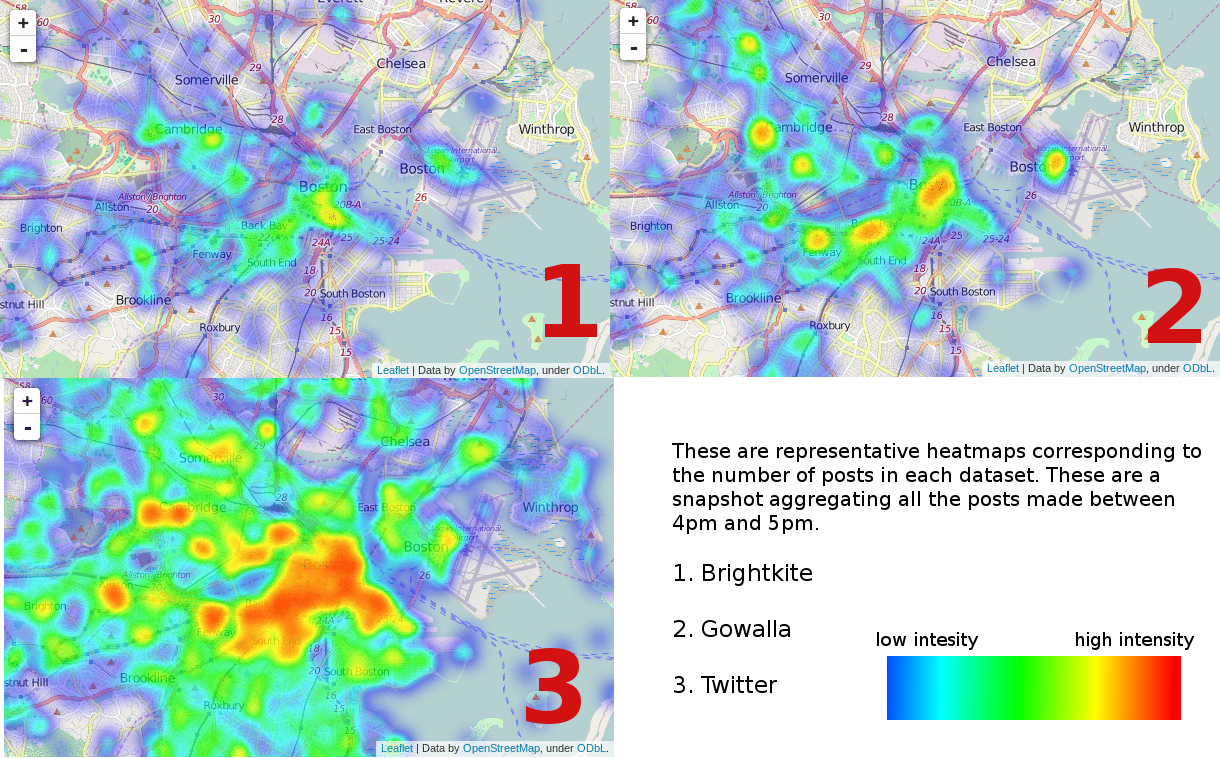
\includegraphics[scale=0.5]{heatmap.png}
\begin{tabular}{c | c | c | c | c }
Service & \# of users & \# of posts & $\frac{posts}{users}$ & duration\\
\hline
Brightkite & 1,383 & 31,928 & 23 & 917 days\\
Gowalla & 2,395 & 39,398 & 16 & 547 days\\
Twitter & 39,540 & 632,990 & 16 & 291 days
\end{tabular}
%\includegraphics[scale=0.5]{postsperday_p.png}
%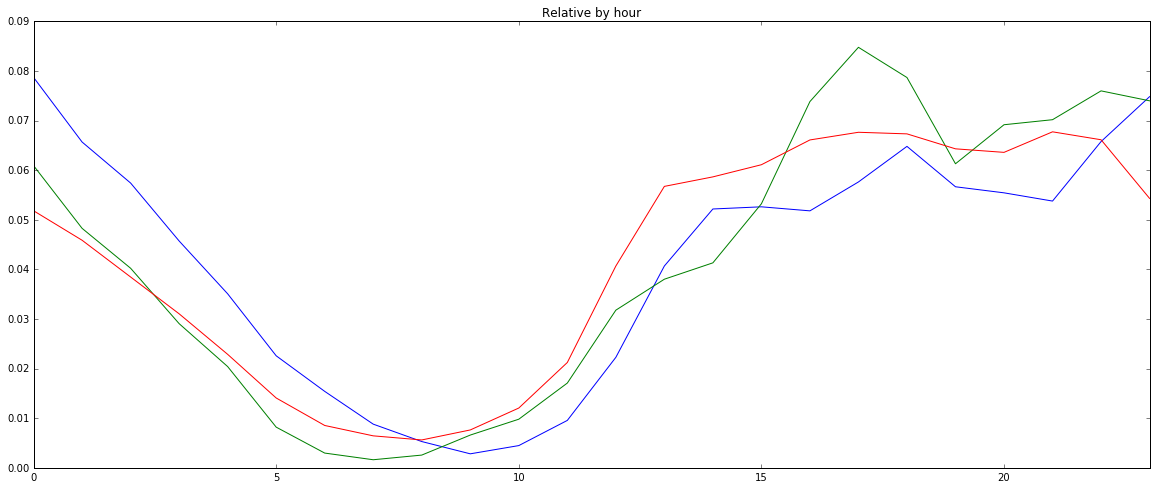
\includegraphics[scale=0.5]{postsbyhour.png}
%also include table of numbers
\section{Segmentation}
%Using the OpenStreetMap data, each Twitter post was associated with the closest intersection. The chart shows the most popular twenty-five intersections. 
%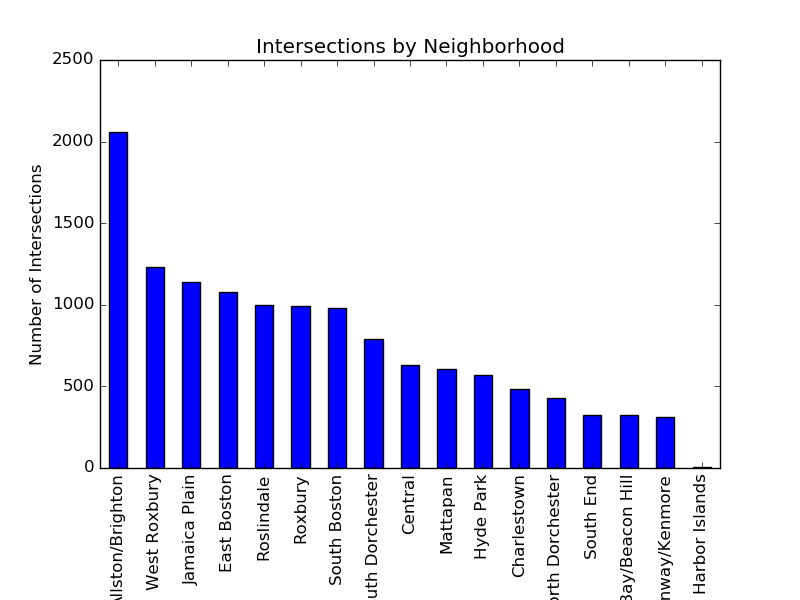
\includegraphics[scale=1.2]{numberofintersections.png}
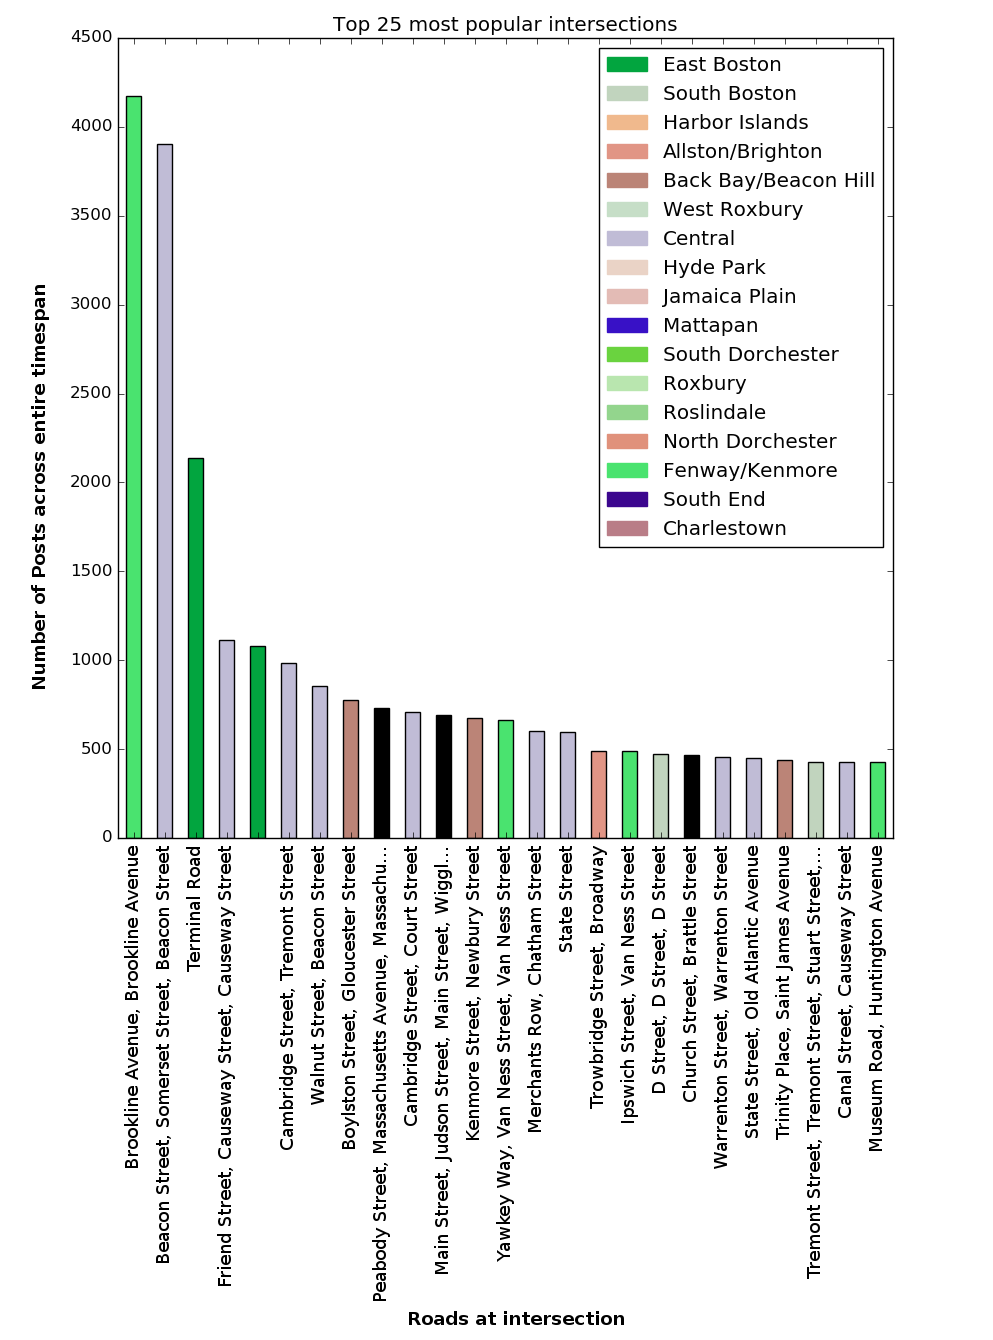
\includegraphics[scale=0.58]{popularintersections.png}
Using the OpenStreetMap data, each Twitter post was associated with the closest intersection. The chart shows the most popular twenty-five intersections. 
%use popular intersection chart here

\section{Intersection Estimation}
\textit{Capture \& Recapture}. This type of sampling was first used when measuring animals in traps. Trappers would mark animals and then count how many of these animals returned to derive an estimate of the total population. This is represented in the following formulation: $$\hat{N} = \frac{Kn}{k}$$ where $\hat{N}$ is the estimation of the total population, $n$ is the number of users during the first month, $K$ is the number of users during the second month, and $k$ is the number of users from the first month that are observed during the second month. With this formulation, we can derive estimations for the number of social media users that post near an intersection per month. 
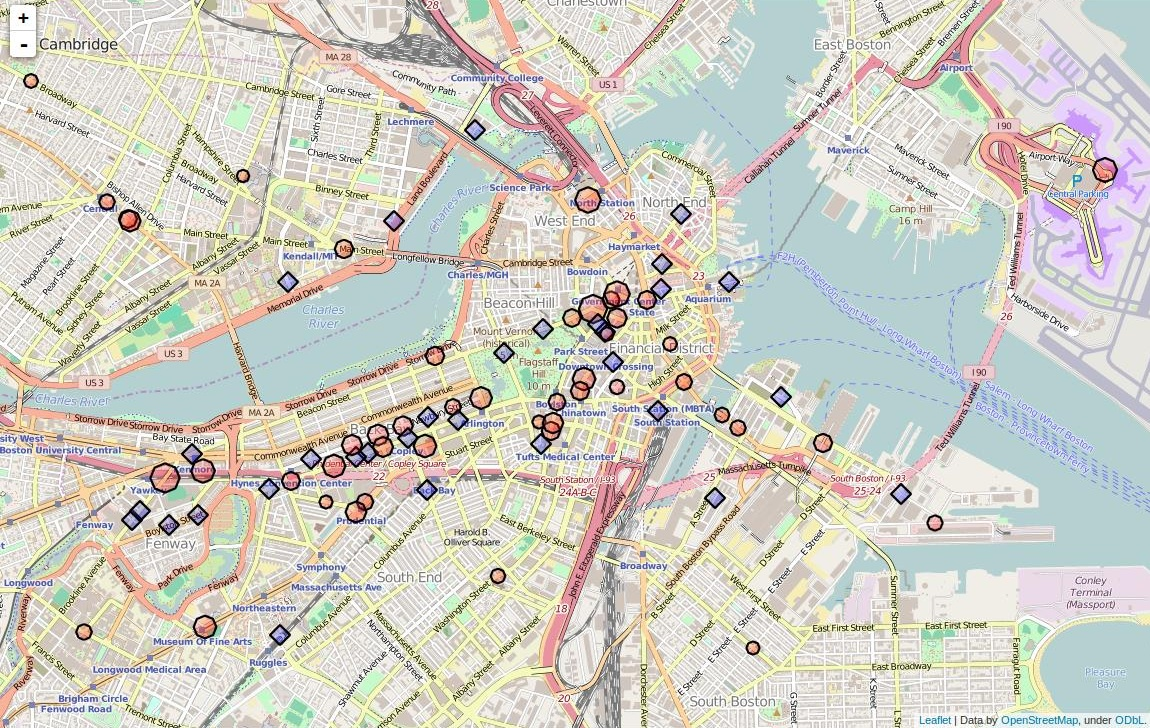
\includegraphics[scale=0.55]{estimate.jpg}
We discovered only 94 intersections, of the almost 25,000, had five or more visitors each month. Only 57 of these intersections had visitors that returned during the capture/recapture period. The \red{red markers} show the intersections that estimates could be computed, scaled with the $\log_2$ function. The \blue{blue markers} show the intersections that did not have returning users. Fenway park had that max estimate with approximately 12,000 visitors per month. 
\section{Data Provenance}
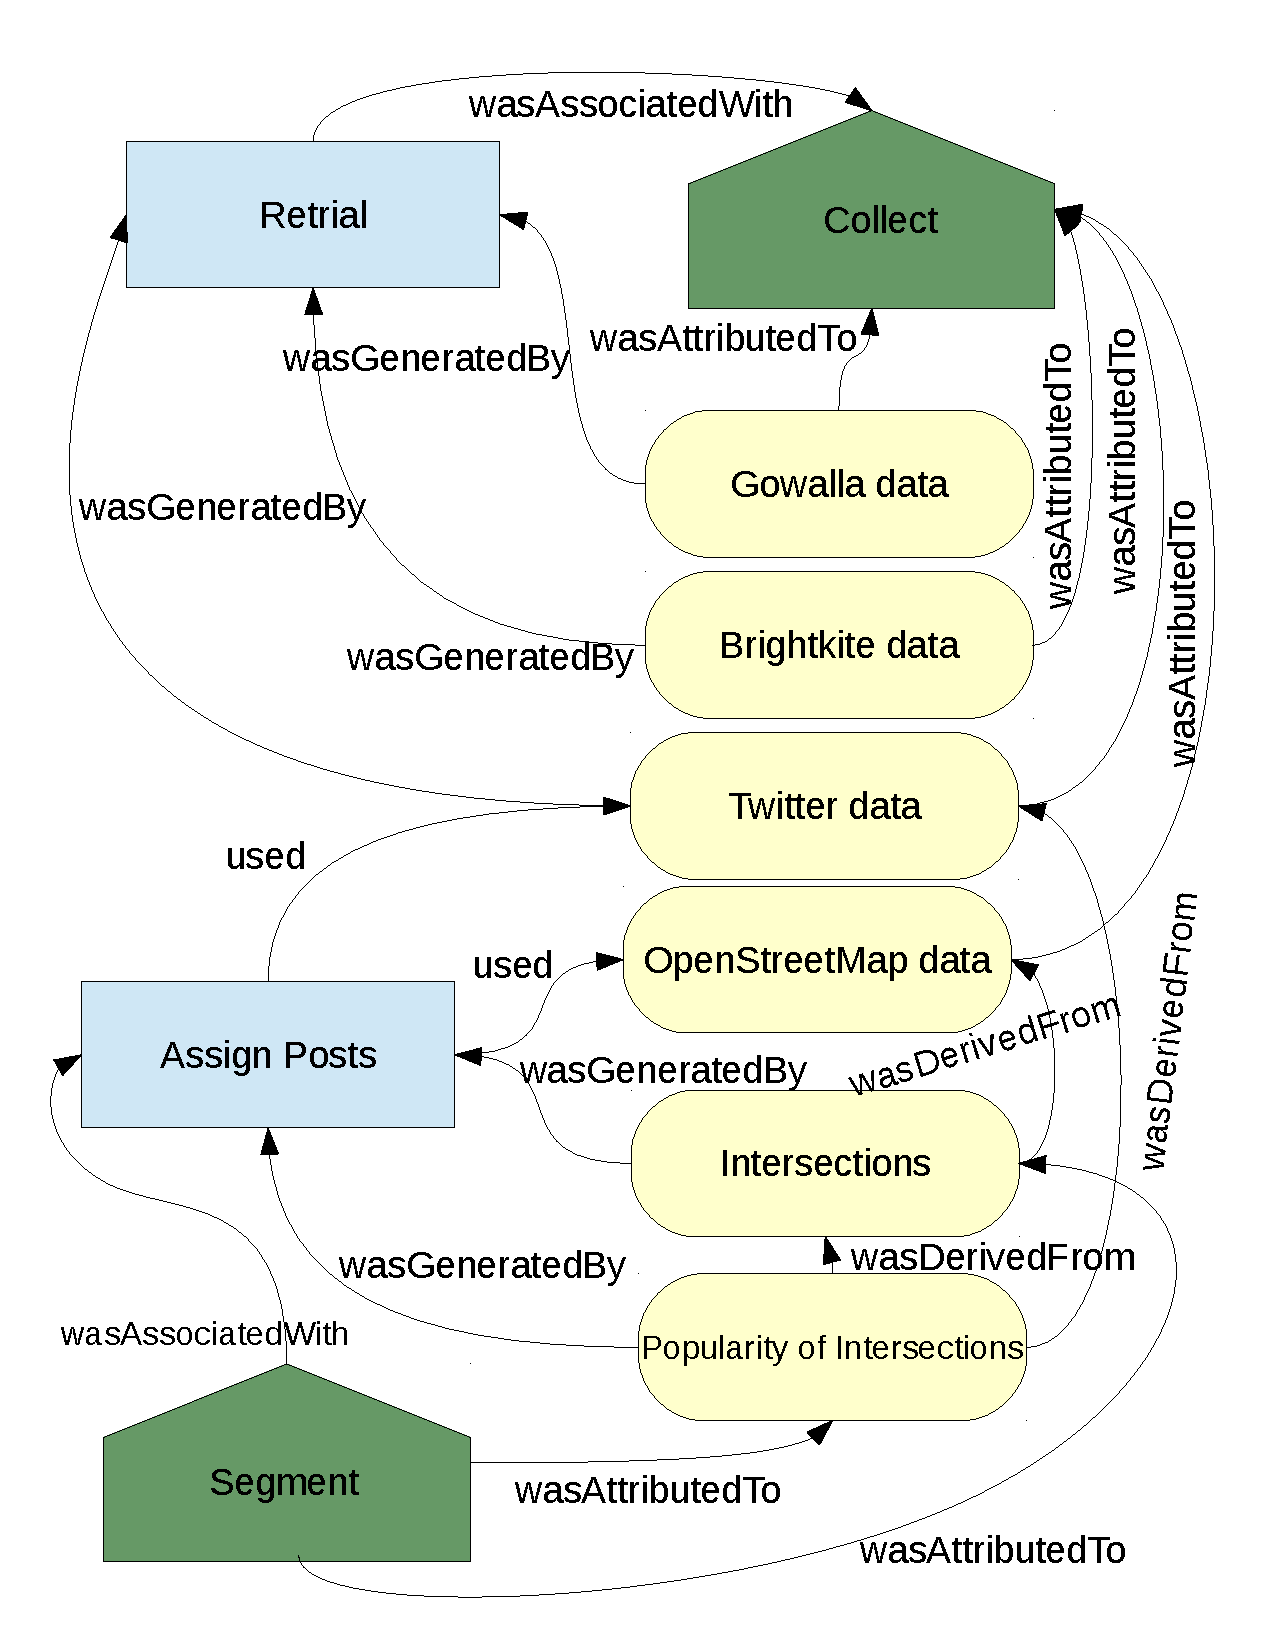
\includegraphics[scale=1]{prov.pdf}
We use six (two of them derived) \dataset{datasets} denoted in \dataset{yellow}, two \agent{agents} in \agent{green}, and two \activity{activities} in \activity{blue}. Excluded from this chart is the provenance information for the scripts that generate the visualizations and some other statistics. 

\section{Conclusions}
Although the social media data consisted of many posts, only a fraction of the intersections had data spanning the entire collection period. Of these intersections, only a fraction had entire data to compete the estimate via the capture \& recapture method. Future work will be to include the Brightkite and Gowalla datasets in the estimation of intersection occupancy and analyzing flow problems associated with pedestrian traffic.

\end{poster}
\end{document}
